\section{Alloy Code}
\label{sec:alloy}%
\begin{lstlisting}[language=alloy,label={lst:alloy_code}]
	open util/ordering[DateTime]
// Alloy model for CodeKataBattle platform - Entities and Facts
abstract sig  BattleState{}
one sig OpenBattle extends BattleState{}
one sig StartedBattle extends BattleState{}
one sig InProgressBattle extends BattleState{}

abstract sig TournamentState{}
one sig OpenTournament extends TournamentState{}
one sig ClosedTournament extends TournamentState{}
one sig InProgressTournament extends TournamentState{}


enum BadgeEnum{ParticipationBadge, GroupPowerBadge, DoubleDigitScoreBadge}

sig Badge{
    badgeType: one BadgeEnum
}


// Signatures
abstract sig User{
    username: one Int
}


sig Student extends User{
    sBadges: set Badge
}


sig Educator extends User{

}

sig Score{
    student: one Student,
    value: Int,
    rank: Int
}


sig Team{
    members: set Student,
    size: Int,
    score: Int // Punteggio del team nella battle
}


sig Battle{
    teams: disj set Team,
    min_size: Int,
    max_size: Int,
    state: one BattleState,
}


sig Tournament{
    participants: set Student,
    leaderboard: set Score,
    administrators: set Educator,
    battles: disj set Battle,
    tState: one TournamentState,
    tBadges: disj set Badge
}

// ------------------------ USER RELATED FACTS ------------------------

// Req: every user as an unique usernanme

fact uniquesername{
    all u1, u2: User | u1!=u2 implies u1.username != u2.username
}

// ------------------------- TOURNAMENT RELATED FACTS

// A score can't be in two different tournaments

fact noDoubleScore{
    all t1, t2: Tournament, s1: t1.leaderboard, s2: t2.leaderboard|t1!=t2 implies s1 != s2
    
}


// Links the score in the tournament with the participants in the same tournament

fact studentInTournamentMatchesScore {
    all t: Tournament | t.participants = (t.leaderboard.student)
}

// In a tournament, a student is linked to only one score

fact singleStudentScore{
    all tournament: Tournament, s1, s2: tournament.leaderboard | s1 != s2 implies s1.student != s2.student
}


// Tournament needs to have at least one administrator

fact numAdministrators{
    all t: Tournament | #t.administrators > 0
}

// ---------------------- TEAM RELATED FACTS
// Just some general variable check

fact generalTeamReq{
    all team: Team | #team.members <= team.size and team.size > 0 and team.score >= 0 and #team.members > 0
    
}

// The size defined for the team must be in battle constraint and Num of members is at least minimum in a team

fact correctSize{
    all battle: Battle, team: battle.teams | team.size >= battle.min_size and team.size <= battle.max_size and #team.members >= battle.min_size
}

// The students in a team must be all relative to the same tournament

fact possibleTeam{
    all t: Tournament, b: t.battles, team : b.teams, m: team.members | m in t.participants 
}

// Teams must be linked to a battle

fact teamBattleRel{
    all team: Team| one battle: Battle | team in battle.teams
}

// Students in a battle must be in only one team

fact oneTeamPerStudent{
    all battle: Battle, team1, team2: battle.teams | team1 != team2 implies (all s1: team1.members, s2: team2.members | s1 != s2)
}

// ----------------------- BATTLE RELATED FACTS

fact generalBattleReq{
    all battle: Battle | battle.min_size <= battle.max_size and battle.min_size > 0
}

// Battle are related to tournament

fact battleTournamentRel{
    all battle: Battle | one tournament: Tournament | battle in tournament.battles
}

// ----------------------- SCORE RELATED FACTS

// general req

fact generalScoreReq{
    all score: Score | score.value >= 0 and score.rank > 0
}

// All ranks are in order given their score

fact ranksAreInSuccession {
    all t: Tournament, s: t.leaderboard | s.rank > 0 and s.rank <= #t.leaderboard
    all t: Tournament, s1, s2: t.leaderboard | s1 != s2 implies s1.rank != s2.rank
    all t: Tournament | lone s: t.leaderboard | s.rank = 1
    all t: Tournament | lone s: t.leaderboard | s.rank = #t.leaderboard
}

//For every two students in the participant sets, a student with a higher score in a tournament has a lower rank

fact studentsWithHigherScoreHaveLowerRank{
    all t: Tournament, s1, s2: t.leaderboard | s1 != s2 implies ((s1.value >= s2.value iff s1.rank <= s2.rank)) //and (s1.value = s2.value implies s1.rank = s2.rank))

}

// A score is linked to a torunament

fact scoreLinkedTournament{
    all score: Score | some tournament: Tournament | score in tournament.leaderboard
}

// the score is the some of the scores acquired in the challenges

fact consistentScore{
    all t: Tournament, s: t.leaderboard | s.value = (sum team: {team: Team | s.student in team.members && (some battle: t.battles | team in battle.teams)} | team.score)
}


// ----------------------- BADGE RELATED FACTS

// Badges exists withnin tournament scope

fact badgeTournamentRel{
    all b: Badge | some t: Tournament | b in t.tBadges
}

// Badges in a tournament are all different

fact allDiffBadgesT{
    all t: Tournament, b1, b2: t.tBadges | b1 != b2 implies b1.badgeType != b2.badgeType
}

// Badges of a student are all different

fact allDiffbadgesS{
    all s: Student, b1, b2: s.sBadges | b1 != b2 implies b1.badgeType != b2.badgeType
}

// A student can have a badge if he was in a tournament where that badge was acquirable

fact coherenceAcq{
    all s: Student, b: Badge | some t: Tournament | b in s.sBadges implies (b in t.tBadges && s in t.participants)   
}

// Student that are in a tournament where participationBadge is available, must have a partecipationBadge

fact participationsBadgeAcq{
    all t: Tournament, s: t.participants, b: t.tBadges | b.badgeType = ParticipationBadge implies (one b2: Badge | b2.badgeType = ParticipationBadge && b2 in s.sBadges)
}

// Student in a tournament with GroupPower Badge can acquire it if conditions are satisfied

fact groupBadgeAcq{
    all t: Tournament, badge: t.tBadges, battle: t.battles, team: battle.teams |
        (badge.badgeType = GroupPowerBadge && #team.members >= 2) implies (all s: team.members | one b2: Badge | b2.badgeType = GroupPowerBadge && b2 in s.sBadges)
}

fact groupBadgeAcqR{
    all s: Student, badge: s.sBadges | badge.badgeType = GroupPowerBadge implies (some team: Team | #team.members > 2 && s in team.members)
}

// Student in a tournament with DoubleDigitScoreBadge can acquire it if conditions are satisfied

fact DoubleDigitScoreBadgeAcq{
    all t: Tournament, badge: t.tBadges, score: t.leaderboard | (badge.badgeType = DoubleDigitScoreBadge && score.value > 9) implies 
    (one b2: Badge | b2.badgeType = DoubleDigitScoreBadge && b2 in score.student.sBadges)
}

fact DoubleDigitScoreBadgeAcqR{
    all s: Student, badge: s.sBadges | badge.badgeType = DoubleDigitScoreBadge implies (some score: Score | s = score.student && score.value > 9)
}
\end{lstlisting}
\section{Simulations}
\label{sec: sim}%
Below is presented a simulation of the built model.\\
The world has been simulated forcing Alloy to generate more entities (Tournaments, Battles, Teams, Badges, etc.) in order to give a deeper insight of the model.
%Two simulations of the built model are presented below.\\
%The first simulation is the simpler one, it's useful to understand the general ideas behind the model and the relations between elements.\\
%The second world is more complex as it was simulated forcing Alloy to generate more entities (Tournaments, Battles, Teams, Badges, etc.) 
%in order to give a deeper insight of the model.

\begin{sidewaysfigure}
	\begin{figure} [H]
		\begin{center}
			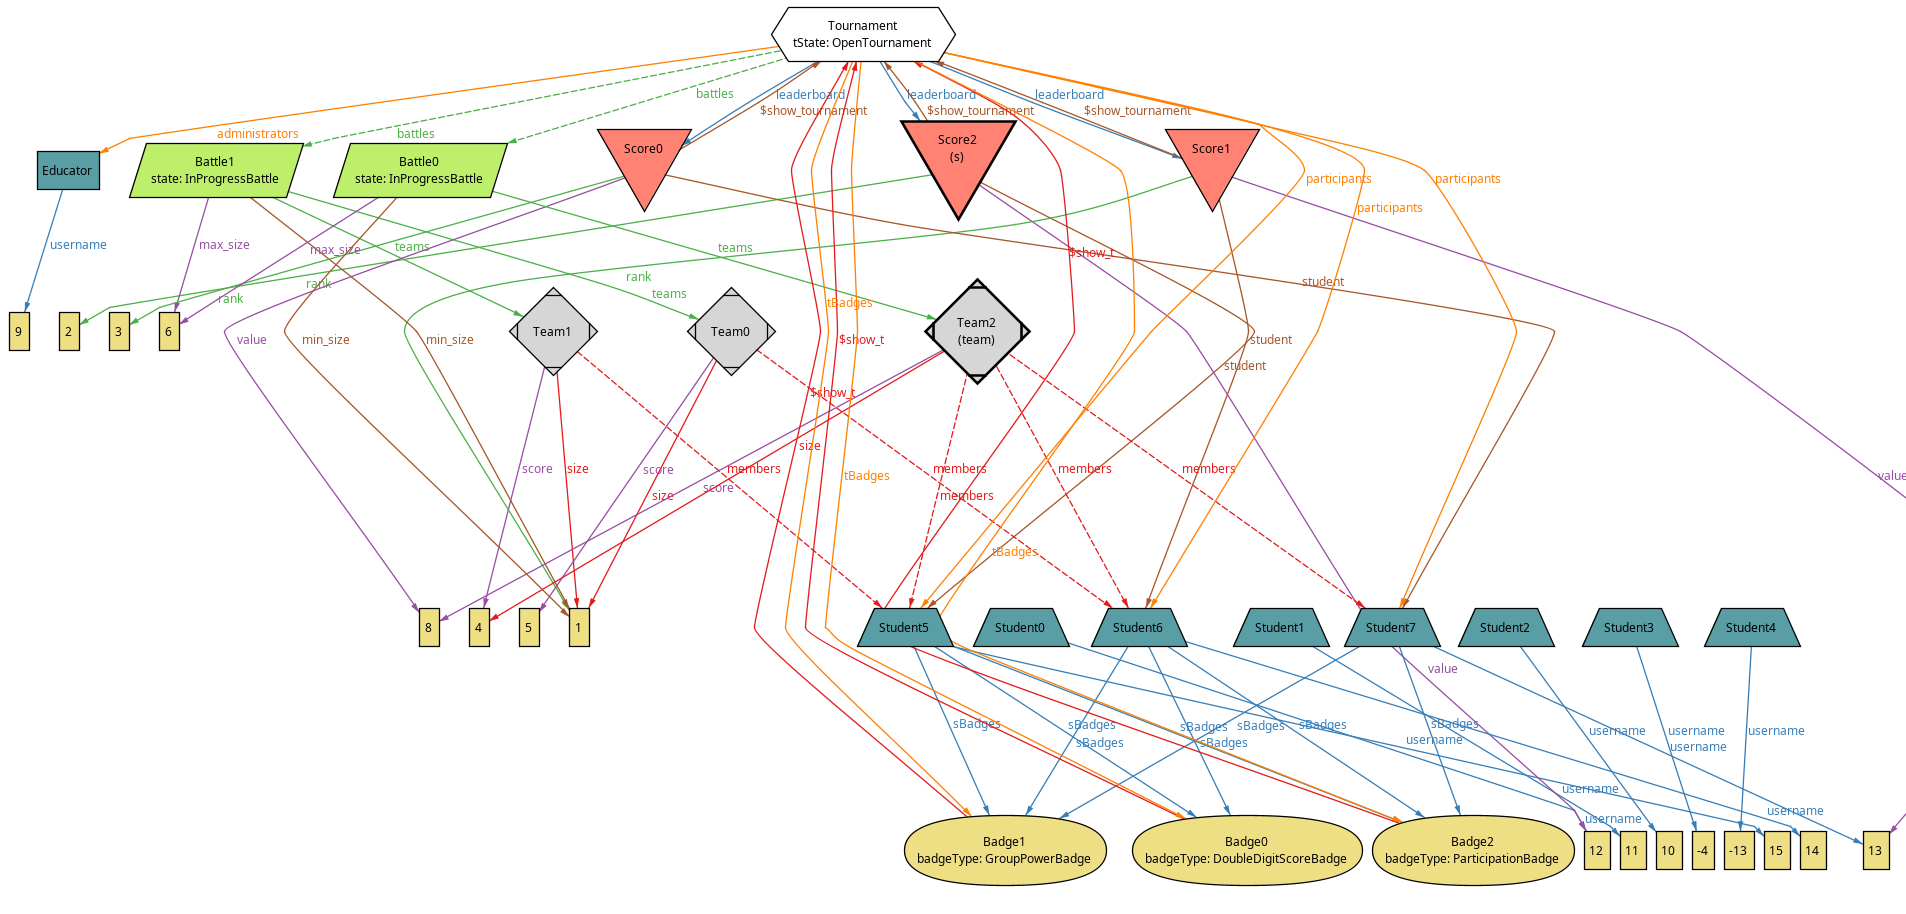
\includegraphics[width=1\linewidth]{Images/AlloyWorld.png}
			\caption{Alloy World .}
			\label{fig: alloy_world}
		\end{center}
	\end{figure}
\end{sidewaysfigure}
%
%\begin{sidewaysfigure}
%	\begin{figure} [H]
%		\begin{center}
%			\includegraphics[width=1\linewidth]{graphs/worldWithManyAppointments}
%			\caption{More complex world.}
%			\label{fig: many_appointments_world_alloy}
%		\end{center}
%	\end{figure}
%\end{sidewaysfigure}